\begin{figure}[ht]
    \centering
    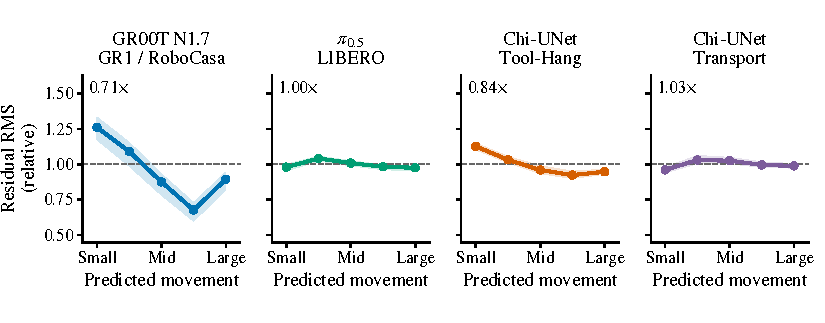
\includegraphics[width=\linewidth]{mse_action_magnitude.pdf}
    \caption{\textbf{Movement size and MSE fitting residuals.}
    Observations are grouped into within-task quintiles of predicted movement
    magnitude after undoing action normalization. The vertical axis shows
    continuous-action residual RMS relative to each task's pooled RMS;
    tasks are equally weighted. Bands are episode-bootstrap 95\% confidence
    intervals. Annotations compare the largest- and smallest-movement groups.
    Target actions are not used to define the groups.}
    \label{fig:mse-action-magnitude}
\end{figure}
